%
% File acl2015.tex
%
% Contact: car@ir.hit.edu.cn, gdzhou@suda.edu.cn
%%
%% Based on the style files for ACL-2014, which were, in turn,
%% Based on the style files for ACL-2013, which were, in turn,
%% Based on the style files for ACL-2012, which were, in turn,
%% based on the style files for ACL-2011, which were, in turn, 
%% based on the style files for ACL-2010, which were, in turn, 
%% based on the style files for ACL-IJCNLP-2009, which were, in turn,
%% based on the style files for EACL-2009 and IJCNLP-2008...

%% Based on the style files for EACL 2006 by 
%%e.agirre@ehu.es or Sergi.Balari@uab.es
%% and that of ACL 08 by Joakim Nivre and Noah Smith

\documentclass[11pt]{article}
\usepackage{acl2015}
\usepackage{times}
\usepackage{url}
\usepackage{latexsym}
\usepackage{setspace}
% \doublespacing
%\setlength\titlebox{5cm}
\usepackage{graphicx}
\usepackage{xcolor}
%\usepackage{natbib}
\usepackage{booktabs}

\newcommand{\wacomment}[1]{\textcolor{blue}{[#1 \textsc{--Waleed}]}}
\newcommand{\dkcomment}[1]{\textcolor{red}{[#1 \textac{--DK}]}}

% You can expand the titlebox if you need extra space
% to show all the authors. Please do not make the titlebox
% smaller than 5cm (the original size); we will check this
% in the camera-ready version and ask you to change it back.


\title{The AI2 Submission at The Rich Context Competition}
%Extracting Datasets and Metadata from Social Science Publications}

\author{Daniel King, Waleed Ammar, Iz Beltagy, Christine Betts \\ \textbf{Suchin Gururangan and Madeleine van Zuylen} \\
\\
Allen Institute for Artificial Intelligence, Seattle, WA, USA\\
{\tt daniel@allenai.org}\\}


\date{}



\begin{document}
\maketitle

\section{Introduction}
The Allen Institute for Artificial Intelligence (AI2) is a non-profit research institute founded by Paul G. Allen with the goal of advancing artificial intelligence research for the common good.
One of the major undertakings at AI2 is to develop an equitable, unbiased software platform (Semantic Scholar)\footnote{\url{www.semanticscholar.org}} for finding relevant information in the scientific literature.
Semantic Scholar extracts meaningful structures in a paper (e.g., images, entities, relationships) and links them to other artifacts when possible (e.g., knowledge bases, GitHub repositories), hence our interest in the rich context competition (RCC).
In particular, we participated in the RCC in order to explore methods for extracting and linking datasets used in papers.
At the time of this writing, Semantic Scholar comprehensively covers the computer science and biomedical literature, but we plan to expand our coverage in 2019 to other scientific areas, including social sciences.

In the following sections, we describe our approach to the three tasks of the RCC competition: extracting datasets used in publications (Section \ref{sec:datasets}), research area prediction (Section \ref{sec:areas}) and research method extraction (Section \ref{sec:methods}).

\section{Dataset Extraction and Linking}\label{sec:datasets}
This task focuses on identifying datasets used in a scientific paper. 
Datasets which are merely mentioned but not used in the research paper are not of interest.
This task has two sub-tasks:
\begin{enumerate}
    \item Citation prediction: extraction and linking to a provided knowledge base of \emph{known datasets}, and 
    \item Mention prediction: extraction of both \emph{unknown and unknown} dataset mentions.
\end{enumerate}

\paragraph{Provided Data.}
The provided knowledge base of known datasets includes approximately 10K datasets used in social science research.
Many of the datasets in the knowledge base are specific years or sections of larger surveys, e.g.,
\begin{itemize}
    \item  Monitoring the Future: A Continuing Study of the Lifestyles and Values of Youth, 1980 
    \item Monitoring the Future: A Continuing Study of the Lifestyles and Values of Youth, 1983
    \item Monitoring the Future: A Continuing Study of American Youth (12th-Grade Survey), 1996
\end{itemize}
The high textual similarity between different datasets in the knowledge base makes the linking task more challenging.

In the first phase of the RCC, organizers provided participants with 5K papers, partially annotated with dataset usage to serve as training data.
For each paper, the full text, metadata, and PDF file were provided.
For each annotation, the paper ID and the corresponding dataset ID in the knowledge base were provided.
For most annotations, the textual mentions in the paper were also provided, but the position of the mention in the paper text was not specified. This means that for a mention that appears multiple times in a paper, it is ambiguous which of these mentions is actually the reference to the dataset that has been labeled. In order to actually label the text in the paper, we need to search the paper for the annotated mention, and if the mention appears multiple times, it is not clear which of these are valid examples of dataset usage in a paper.
Approximately 10\% of the datasets in the knowledge base were linked one or more times in the provided corpus of 5K papers.

\begin{figure*}[h]
\centering
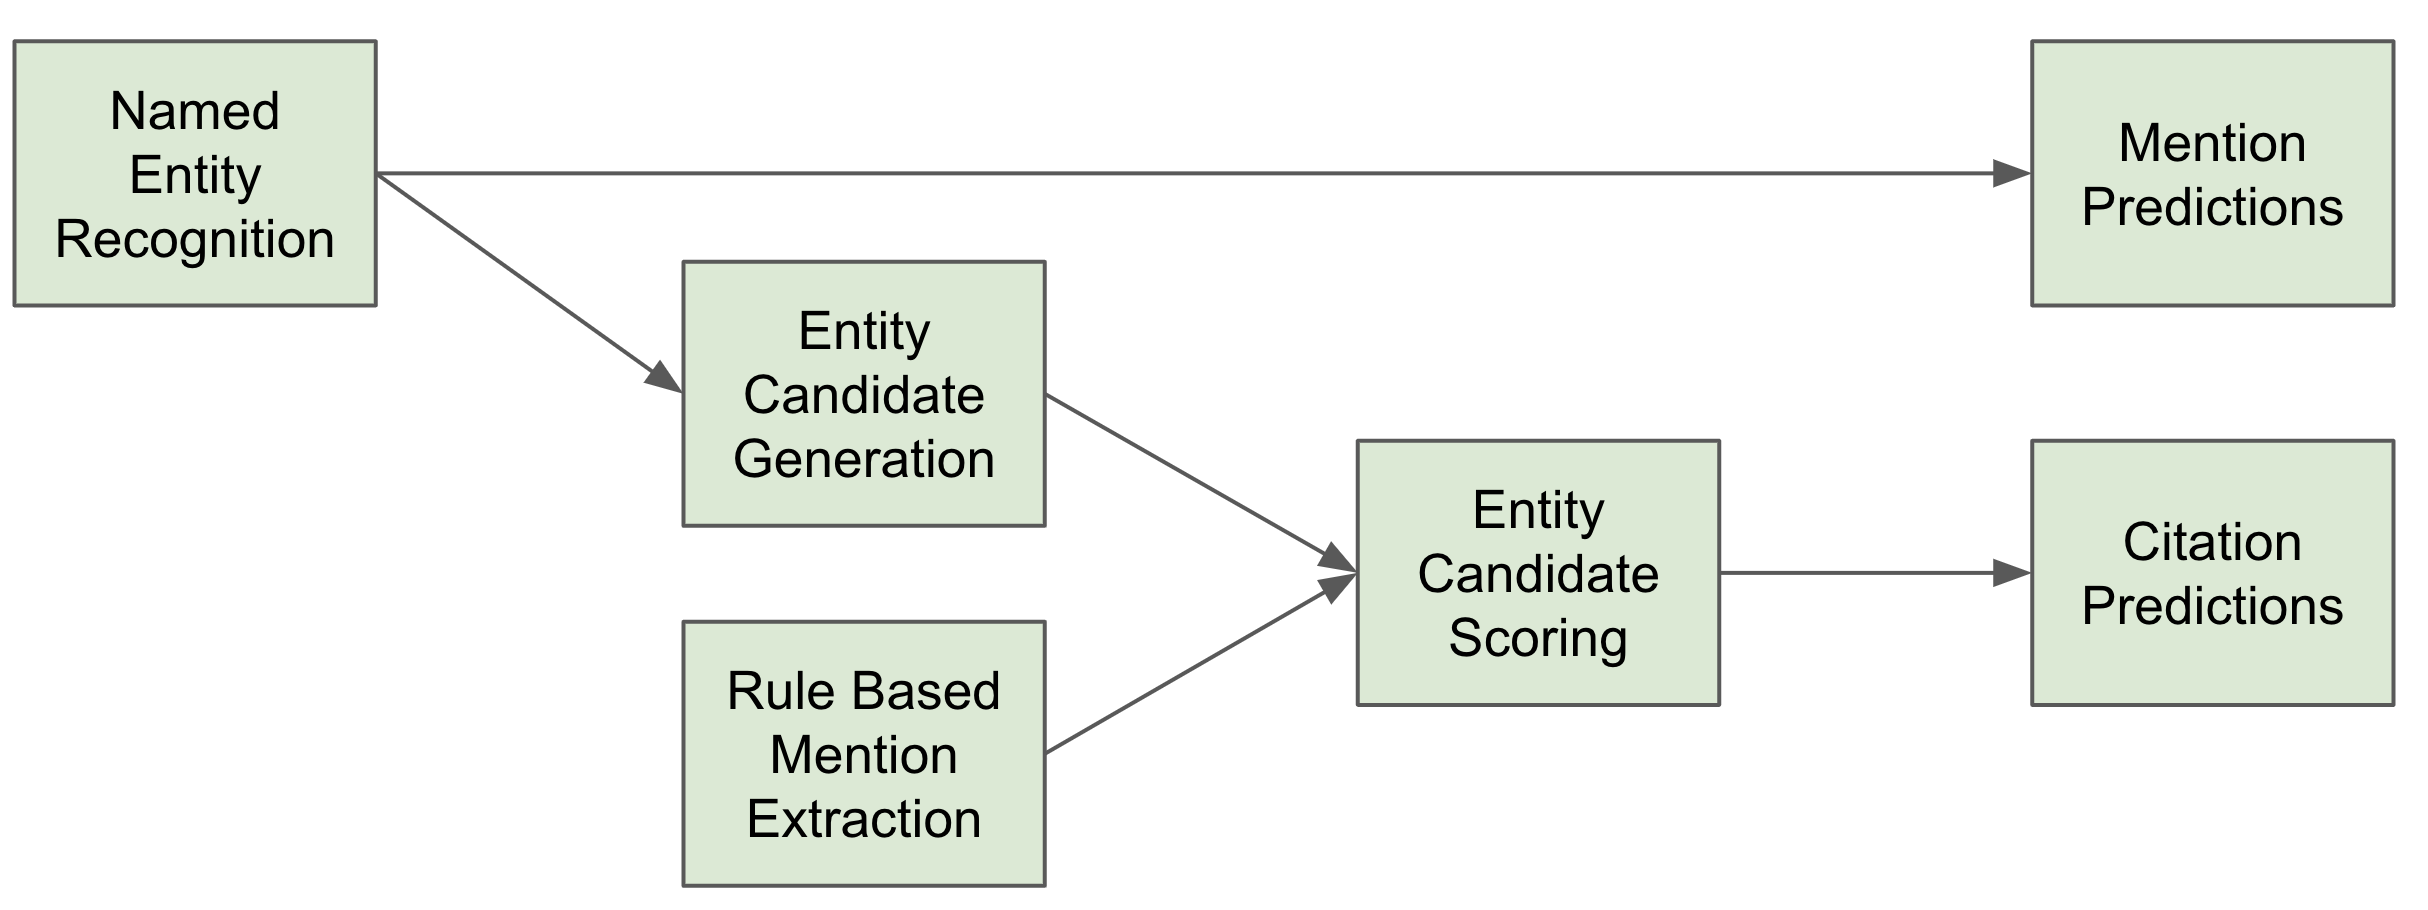
\includegraphics[width=13cm]{datasets.png}
\caption{Overview of our approach to dataset extraction and linking.}\label{fig:datasets}
\end{figure*}

We provide a high-level overview of our approach in Figure \ref{fig:datasets}.
First, we use a named entity recognition (NER) model to predict dataset mentions. 
For each mention, we generate a list of candidate datasets from the knowledge base. 
We also developed a rule based extraction system which searches for dataset mentions seen in the training set, adding the corresponding dataset IDs in the training set annotations as candidates.
We then use a binary classifier to predict which of these candidates is a correct dataset extraction.

Next, we describe each of the sub-components in more detail.

\paragraph{Mention and Candidate Generation.}
We first constructed a set of rule based candidate citations by exact string matching mentions and dataset names from the provided knowledge base. We found this to have high recall on the provided development fold and our own development fold that we created. However, after our test submission, it became clear that there were many datasets in the actual test set that did not have mentions in the provided knowledge base.

To address this limitation, we developed an NER model to predict additional dataset mentions.
For NER, we use a bi-LSTM model with a CRF decoding layer, similar to \cite{Peters2018DEEPCW}, and implemented using the AllenNLP framework.\footnote{\url{https://github.com/allenai/allennlp/blob/master/allennlp/models/crf_tagger.py}}
In order to train the NER model, we automatically generate mention labels by string matching mentions in the provided annotations against the full text of a paper.
This results in noisy labeled data, because it was not possible to find all correct mentions this way (e.g., some dataset mentions were not annotated), and the same string can appear multiple times in the paper, while only some are correct examples of dataset usage.

We limit the percentage of negative examples (i.e., sentences with no mentions) used in training to 50\%, and use 40 words as the maximum sentence length.
We use 50-dimensional Glove word embeddings \cite{Pennington2014GloveGV}, 16-dimensional character embeddings with 64 CNN filters of sizes (2, 3, 4).
The CNN character encoder outputs 128-dimensional vectors.
We optimize model parameters using ADAM \cite{Kingma2014AdamAM} with a learning rate of 0.001.

In order to generate linking candidates for the NER mentions, we score each dataset based on TF-IDF weighted token overlap between the mention text and the dataset title. For a given mention, many dataset titles can have a non-zero overlap score, so we take the top 30 scoring candidates for each mention as the linking candidates for that mention.

\paragraph{Candidate Linking.}
The linking model takes as input a dataset mention, its context, and one of the candidate datasets in the knowledge base, and outputs a binary label.
We use a gradient boosted trees classifier using the  XGBoost implementation.\footnote{\url{https://xgboost.readthedocs.io/en/latest/}}
We use the following features:
prior probability of entity, prior probability of entity given mention, prior probability of mention given entity, whether a year appears in the mention context and in the dataset title, mention length, mention sentence length, whether the mention is an acronym, estimated section title of the mention, overlap between mention context and dataset keywords provided in the knowledge base, and the TF-IDF weighted token overlap.
We note that it is possible to predict zero, one or multiple dataset IDs for the same mention.

\paragraph{Results.}
First, we report the results of our NER model in Table \ref{tab:ner_results}. 
Since it is easy for the model to memorize the dataset mentions seen at training time, we created disjoint train, development, and test sets based on the paper--dataset annotations provided for the competition.
In particular, we sort datasets by the number of papers they appear in, then process one dataset at a time.
For each dataset, we choose one of the train, development or test splits at random and add the dataset to either the train, development or test sets, along with all papers which mention that dataset.
When there is a conflict, (e.g., a paper $\mathbf{p}$ has already been added to the train split when processing an earlier dataset $\mathbf{d_1}$, but it is also associated with a later dataset $\mathbf{d_2}$), the later dataset $\mathbf{d_2}$ along with all papers associated with it are added to the same split as $\mathbf{d_1}$. For any further conflicts, we prefer to put papers in the development split over the train split, and the test split over the development split.

We also experimented with adding ELMo embeddings \cite{Peters2018DEEPCW}, but it significantly slowed down training and decoding which would have disqualified our submission due to the runtime requirements of the competition. As a result, we decided not to include ELMo embeddings in our final model.

\begin{table}[t]
\centering
% \renewcommand{\arraystretch}{1.2}
\setlength{\tabcolsep}{2pt}
\begin{tabular}{@{}cccc@{}}
\toprule
                  & prec. & recall & F1 \\ \midrule
dev set           & 53.4    & 50.3 & 51.8 \\ 
test set          & 50.7    & 41.8 & 45.8 \\ \bottomrule
\end{tabular}
\caption{NER precision, recall and F1 performance (\%) on the development and test sets.}
\label{tab:ner_results}
%\vspace{-10pt}
\end{table}

\begin{table}[t]
\centering
\setlength{\tabcolsep}{2pt}
\begin{tabular}{@{}cccc@{}}
\toprule
                  & prec. & recall & F1 \\ \midrule
phase 1 holdout   & 35.7  & 19.6 & 25.3 \\ 
phase 2 holdout   & 39.6  & 18.8 & 25.5 \\ \bottomrule
\end{tabular}
\caption{End-to-end precision, recall, and F1 performance (\%) for dataset prediction on the phase 1 and phase 2 holdout sets. Note that the phase 1 holdout results are for citation prediction, while the phase 2 holdout results are for mention prediction.}
\label{tab:test_results}
\end{table}

We report the end-to-end performance of our approach (on the development set provided by the organizers in the first phase) in Table \ref{tab:e2e_results}. This is the performance after using the linking classifier to predict which candidate mention, dataset pairs are correct extractions.
We note that the development set provided in phase 1 ended up having significantly more overlap with the training data than the actual test set did. As a result, the numbers reported in Table \ref{tab:e2e_results} are not indicative of test set performance. End to end performance from our phase 2 submission can be seen in Table \ref{tab:test_results}. This performance is reflective of our focus on the linking component of this task. Aside from the competition development set, we also used a random portion of the training set as an additional development set.
The initial model only uses a dataset frequency feature, which gives a baseline performance of 38.4 F1. Adding p(d $\mid$ m) and p(m $\mid$ d), which are the probability of entity given mention and probability of mention given entity improves the performance ($\Delta = 2.3$ F1).
Year matching helps disambiguate between different datasets in the same series, which was found to be a major source of errors in earlier models ($\Delta = 2.8$ F1).
Aggregating mentions for a given dataset, adding mention and sentence length features, adding an is acronym feature, and further hyper-parameter tuning improve the results ($\Delta = 12.5$ F1).
Adding examples in the development set while training the model results in further improvements ($\Delta = 2.8$ F1).
Finally, adding the NER-based mentions significantly improves recall at the cost of lower precision, with a positive net effect on F1 score ($\Delta = 0.7$ F1).

\begin{table}[t]
\centering
% \renewcommand{\arraystretch}{1.2}
\setlength{\tabcolsep}{2pt}
\begin{tabular}{@{}lccc@{}}
\toprule
                  & prec. & recall & F1 \\ \midrule
baseline               & 28.7 & 58.0 & 38.4 \\
+ p(d $\mid$ m), p(m $\mid$ d)  & 39.6 & 42.0 & 40.7 \\
+ year matching        & 35.1 & 57.0 & 43.5 \\
+ aggregated mentions, tuning  & & & \\
\quad and other features & 72.5 & 45.0 & 55.5 \\
+ dev set examples     & 77.0 & 47.0 & 58.3 \\ 
+ NER mentions         & 56.3 & 62.0 & 59.0 \\ \bottomrule
\end{tabular}
\caption{End-to-end precision, recall and F1 performance (\%) for citation prediction on the development set provided in phase 1 of the competition. 
%\dkcomment{The contextual similarity was experimented with and was not included in subsequent models. It was too slow and did not show improvement. I removed it, let me know if you disagree.}
%\wacomment{great, thanks!}
}
\label{tab:e2e_results}
\end{table}

\section{Research Area Prediction}
\label{sec:areas}

\paragraph{Data.}
The second task of the competition is to predict research areas of a paper. 
The task does not specify the set of research areas of interest, nor is training data provided for the task.
After manual inspection of a subset of the papers in the provided test set, the SAGE taxonomy of research, and the Microsoft Academic Graph (MAG) \cite{Shen2018AWS}, we decided to use a subset of the fields of study in MAG as labels.
In particular, we included all fields related to social science or papers from the provided training corpus.
However, since the abstract and full text of papers are not provided in MAG, we only use the paper titles for training our model.
The training data we ended up with included approximately 75K paper titles along with their fields of study as specified in two levels of the MAG hierarchy. We held out about 10\% of the titles for development data. The coarse level (L0) has 7 fields while the more granular one (L1) has 32. 
Fields associated with less than 100 papers were excluded.

\paragraph{Methods.}
For each level, we trained a bi-directional LSTM which reads the paper title and predicts one of the fields in this level.
We additionally incorporate ELMo embeddings \cite{Peters2018DEEPCW} to improve performance. In the final submission, we always predict the most likely field from the L0 classifier, and only report the most likely field from the L1 classifier if it exceeds a certain threshold. It takes approximately 1.5 and 3.5 hours for the L0 and L1 classifiers to converge, respectively.

\paragraph{Results.}

To select a model, we performed a 100 trial random search across model hyper-parameters, evaluated on a held out development set of papers from the Microsoft Academic Graph. Our final model contained 512 hidden dimensions, 2 layers and 0.5 dropout prior to classification. The top performing classifier achieved 84.4\% accuracy on our development set on L0 fields, and 65.2\% accuracy on our development set on L1 fields. 
 
\section{Research Method Extraction}
\label{sec:methods}
\paragraph{Data.}
The third task in the competition is to extract the scientific methods used in the research paper.
Since no training data was provided, we started by inspecting a subset of the provided papers to get a better understanding of what kind of methods are used in social science and how they are referred to within papers. 

\paragraph{Methods.}
Based on the inspection, we designed regular expressions which capture common contextual patterns as well as the list of provided SAGE methods. 
In order to score candidates, we used a background corpus to estimate the salience of candidate methods in a paper.
Two additional strategies were attempted but proved unsuccessful: a weakly-supervised model for named entity recognition, and using open information extraction (openIE) to further generalize the list of candidate methods.

\paragraph{Results.}
We evaluated performance by manually evaluating the output of our extractor for a subset of 50 papers from the provided test set to compute precision. 
Since evaluating recall requires a careful annotation, we resorted to using yield as an alternative metric.
Our final submission for method extraction has a 95\% precision and yield of 1.5 methods per paper on the manually inspected subset of papers.

\section{Conclusion}
This report summarizes the AI2 submission at the RCC competition.
We identify dataset mentions by combining the predictions of an NER model and a rule-based system, use TF-IDF to identify candidates for a given mention, and use a gradient boosted trees classifier to predict a binary label for each candidate mention, dataset pair.
To identify research fields of a paper, we train two multi-class classifiers, one for each of the top two levels in the MAG hierarchy for fields of study.
Finally, we use a rule based system utilizing a dictionary and common patterns, followed by a scoring function which takes into account the prominence of a candidate in foreground and background corpora.

\section{Future Work}
We now provide some possible directions of improvement for each component of our submission. For dataset extraction, the most promising avenue of improvement is to improve the NER model, and the most promising avenue to improve the NER model is to collect less noisy data. We effectively have distantly supervised training data for the NER model, and the first thing to try would be directly annotating papers with dataset mentions to provide a clearer signal for the NER model. For research area prediction, it would help to include signals beyond just the paper title for predicting the field of study. The difficulty here is finding labeled training data that includes richer signals like abstract text and paper keywords. For method prediction, further exploration of using open information extraction is a potential avenue of future research. Additionally, it would be helpful to clarify what exactly is meant by a method, as it is currently unclear what a successful method extraction looks like.

\section*{Acknowledgments}
We would like to thank the competition organizers for their tireless efforts in preparing the data, answering all our questions, doing the evaluations, and providing feedback.
We also would like to thank Zhihong (Siri) Shen for helping us use the MAG data.

% include your own bib file like this:
\bibliographystyle{acl}
\bibliography{acl2015}

%\begin{thebibliography}{}
%\end{thebibliography}

\end{document}

